
% AI进化一定会像人类进化，走过一段波澜壮阔的演进历史。现在所有AI达到的成就都不过是沧海一粟。

% 现在的AI：人类把自己的记忆经验填鸭式输入给AI的一场“盛大表演”，背后是高昂的人力和算力成本。

% 尽管展示出诸多优势，离“有进化能力的生命体”想去甚远，几个致命性问题没有在根本上解决，包括如何感知环境、去中心化训练、在线学习记忆、进化协作能力等等。

% \begin{figure}[h]
%     \vspace{-.5em}
%     \centering
%     \includegraphics[width=0.95\textwidth]{figures/rsi-overview-v7.png}
%     \vspace{-0.2cm}
%     \caption{An Overview of Recursive Self-Improvement.}
%     \label{fig:rsi-stages}
% \end{figure}

%     \includegraphics[width=\textwidth]{figures/rsi-overview-v5.pdf}
%     \captionof{figure}{An Overview of Recursive Self-Improvement.}



\section{Introduction}

% background and emerging of RSI

Recent frontier-model development illustrates several forms of scaling in the improvement pipeline. Kimi K3 and Qwen3.8-Max contain 2.8 trillion and 2.4 trillion parameters, respectively, and each supports a context window of approximately one million tokens~\cite{moonshot2026kimik3,alibaba2026qwen38max}. The development process is also expanding. During the six months preceding GPT-5.6, OpenAI reports that the share of research compute devoted to internal coding inference grew 100-fold and internal agentic token use grew 22-fold, and average daily output tokens per active researcher exceeded twice the previous peak observed with GPT-5.5~\cite{openai2026gpt56}. Scale accumulates across training runs, model-assisted experiments, inference, evaluation, and human validation.

\subsection{Scaling Burdens in Model Development}

Despite the growing use of agentic tools and API-based automation, developers must still determine what to improve, construct the required resources, and establish whether each change works~\cite{nvidia2025aimo,meta_capacity_efficiency_2026}. As AI systems take on more demanding tasks, the cost of scaling this end-to-end development process becomes a bottleneck~\cite{openai2025gdpval,phan2025hle,swebench,yao2024tau}. The following three challenges occur at different stages of the model lifecycle and motivate RSI:



%frontier academic breadth (48.3), Interactive and repository-level tasks

%Traditional AI improvement paradigm (e.g., for human-driven data curation, model architecture design, and training pipeline optimization) is not keeping pace with the expectancy for the near-term arrival of AGI. 

% \begin{figure}[!t]
%     \centering
%     \includegraphics[
%         width=1\linewidth,
%         trim={0cm 0cm 19.6cm 0cm},
%         clip
%     ]{figures/rsi-trend}
%     \caption{The necessity of pursuing RSI for LLMs.}
%     \label{fig:rsi-trend}
% \end{figure}

\noindent$\bullet$ \bfit{Development challenge 1: Resource-intensive foundation-model training.} Foundation-model development remains resource-intensive across data preparation, architecture design, distributed optimization, and evaluation. Kimi K3 activates 16 of 896 experts and reports an approximate 2.5-fold improvement in scaling efficiency over Kimi K2, while Qwen3.8-Max activates 95 billion of its 2.4 trillion parameters~\cite{moonshot2026kimik3,alibaba2026qwen38max}. Sparse activation reduces per-token computation, but training at this scale still couples expert routing, parallelism, multimodal integration, long-context optimization, and systems design. OpenAI further reports that GPT-5.6 Sol designed and ran hundreds of experiments on its speculative-decoding draft model and monitored training through hardware failures and instability. The resulting changes improved token-generation efficiency by more than 15\%~\cite{openai2026gpt56efficiency}. Data quality also matters in addition to quantity. OpenAI's GDPval illustrates that its 1,320 professional tasks required roughly 9,240 expert-hours in total, with contributors averaging more than 14 years of experience~\cite{openai2025gdpval}. The Humanity's Last Exam pipeline logged more than 70,000 submission attempts and sent approximately 13,000 model-stumping questions to expert review before producing a 3,000-question benchmark~\cite{phan2025hle}. Architecture search remains expensive because candidate structures interact with their data, optimization, and hardware regimes. AgentNAS addresses part of this bottleneck by using an LLM to propose a task-specific seed architecture and construct its search space, but candidate selection still depends on combinatorial search under an externally specified objective~\cite{jeong2026agentnas}.


%These disclosures illustrate distinct resource demands; training tokens should not be interpreted as manually annotated examples.

% Pretraining requires engineers to collect and filter data, remove duplication and contamination, balance domains, and optimize distributed training. Qwen3 expanded its pretraining corpus to approximately 36 trillion tokens, compared with 18 trillion for Qwen2.5. Even the highly efficient DeepSeek-V3 required 2.788 million H800 GPU-hours for its reported training run, excluding prior research and ablation experiments. Post-training introduces additional requirements for demonstrations, preference judgments, and reward signals:

\noindent$\bullet$ \bfit{Development challenge 2: Scaling feedback and learning environments.} Synthetic data and reinforcement learning automate parts of capability development, but introduce substantial requirements for generating and evaluating experience, requiring both experience-generation infrastructure and reliable mechanisms for evaluating and retaining updates. For instance, DeepSeek-V3.2 reports a post-training computational budget exceeding 10\% of its pretraining cost~\cite{deepseekai2025deepseekv32pushingfrontieropen}, while NVIDIA's AIMO-2 pipeline generated 3.2 million long-reasoning solutions and 1.7 million tool-integrated solutions, in addition to curating 540,000 problems~\cite{nvidia2025aimo}.




%The challenge therefore extends beyond obtaining more examples: developers must construct diverse tasks, maintain executable environments, and provide feedback that reflects meaningful success. Automatically generating trajectories does not by itself establish that the training distribution covers deployment failures or that its rewards capture the quality users require.

\noindent$\bullet$ \bfit{Development challenge 3: Recurring adaptation after deployment.} Deployed systems consistently introduce changing documents, unfamiliar tools, incomplete context, and workflows involving interdependent actions. Improving such systems requires engineers to manually diagnose failures, revise retrieval and tool interfaces, manage persistent state, and repeat regression testing through discrete, human-led releases. Anthropic reports that agentic workloads use approximately four times as many tokens as ordinary chat, rising to about fifteen times for multi-agent systems because of longer contexts, coordination, environment setup, and end-to-end verification~\cite{anthropic2025research}, while Meta reports that FBDetect identifies thousands of infrastructure regressions each week, and diagnosing one such regression required roughly ten engineer-hours~\cite{meta_capacity_efficiency_2026}.

%Within-task reasoning and persistent memory support adaptation, but neither alone guarantees that experience becomes a validated improvement to future learning or execution.

% Its work on long-running agents further illustrates the importance of


% open-ended environments characterized by distribution shifts, incomplete supervision, and evolving tasks

%\dy{By 2025, global AI compute capacity had reached approximately 17.1 million H100-equivalents, while industry produced more than 90\% of notable AI models \cite{stanford2026aiindex}. As of 2026, frontier language-model training compute is estimated to be growing at roughly $5\times$ per year and training cost at approximately $3.5\times$ per year; moreover, five hyperscalers control about 71\% of global AI compute capacity \cite{epoch2026trends}.}

\subsection{From Development Burden to RSI}

The burdens arise because model improvement remains a sequence of costly, externally coordinated interventions. To address these barriers, RSI inspects whether part of that coordination can become a persistent capability of the system being improved. We define recursive self-improvement (RSI) as an autonomous, closed-loop process in which an AI system identifies its own limitations, develops and validates improvements, and uses the resulting capabilities to improve the improvement process itself. The model evolution paradigm of RSI spans three dimensions: autonomy, efficiency, and innovation. Autonomy expands the system's responsibility from executing a prescribed update to identifying limitations, extracting experience, proposing changes, and validating and retaining successors. Efficiency seeks more validated improvement from data, compute, inference, human review, and rework. Innovation allows the system to search beyond human-prescribed update strategies and feed useful discoveries back into later improvement rounds. These dimensions describe how the full improvement loop is organized and what it can inherit.

% To address the above barriers, recursive self-improvement (RSI) offers a fundamentally different path: an autonomous, closed-loop process in which AI identifies its own limitations, develops and validates improvements, and uses the resulting capabilities to refine the improvement process itself toward the stated goals \zxh{refs}. 

Rather than a particular learning algorithm or a one-off optimization result~\cite{schmidhuber2003godel,zelikman2024stop,zhang2026dgm}, RSI aims to improve both task performance and the mechanisms through which later improvements are discovered and implemented. The following cases illustrate this distinction at two points in the model lifecycle, including foundation-model training and persistent adaptation in software engineering, covered and studied in later sections.


% \zxh{-- table to compare RSI, RL, xxx} 

%Recent advances in foundation models have largely been fueled by massive investments in human labor, computing infrastructure, API-based data generation and evaluation, and large-scale data acquisition and curation \zxh{-- add statistics}. 

%This dependence on large-scale resources remains pronounced at today's capability frontier. 


% \noindent\todo{2.1 Give two example cases: one for the RSI needed in foundation model pre-training; and one for the online learning RSI needed under deployment scenario.}

\noindent$\bullet$ \textbf{Case 1: Foundation-model training.} A conventional experiment loop selects a better checkpoint while leaving the procedure for choosing later experiments unchanged. A-Evolve-Training instead consolidates post-training outcomes into a persistent research policy and discovery log, which a meta-agent revises to guide later workers' recipe choices~\cite{shi2026aevolvetraining}. When development scores improved without corresponding external gains, the system redirected experiments toward data rebalancing and checkpoint selection. The retained policy changes both how successor models are trained and how later improvements are sought. Across four autonomous rounds on a 30B Nemotron model, the external score rose from 0.80 to 0.86, compared with 0.87 for the top human submission~\cite{shi2026aevolvetraining}.

\noindent$\bullet$ \textbf{Case 2: Software-engineering adaptation after deployment.} Repairing a repository changes the software product but may leave the coding agent's recurring failures untouched. Ouroboros instead uses reviewed deployment evidence to propose versioned changes to the agent's tools, context assembly, prompts, and core implementation~\cite{razzhigaev2026ouroboros}. Candidate revisions undergo tests and human review before an accepted version replaces the runtime used for later work. The persistent update improves subsequent coding behavior and changes the mechanism through which later failures are diagnosed and repaired, while experts retain control over consequential corrections and deployment.
%By combining real-world interaction with simulation, world models, and automated feedback loops, RSI may enable AI systems to expand their operational boundaries, reduce the cost of iteration, and achieve sustained capability growth under fixed or limited resources. \zxh{give examples} 

% The capability of RSI is particularly important in \zxh{AI companies that develop foundational models and other companies that deploy AI-based capabilities (e.g., resource-constrained edge, autonomous, and embodied systems)}\cite{zheng2025edgellm,kawaharazuka2025vla}.

%an AI system continually identifies its own limitations, collects or generates targeted experience, improves its models, strategies, tools, or operating environment, and evaluates whether these changes lead to measurable progress \zxh{-- see comment}

% the advantages of RSI

%\dy{For example, there are hard constraints on memory / latency on fixed resources like edge‑side devices, robots and intelligent driving systems. It need self-improvement to become part of the deployed system’s operating capability.}

% \dy{For example, even relatively compact billion-parameter models can exceed the memory or real-time inference budgets of edge devices and robotic platforms, motivating model compression, efficient inference, and on-device adaptation rather than straightforward model scaling\cite{dhar2024edgefootprint}.}

% , where simply deploying larger models is often infeasible

%\bfit{A. What is \RSI: Terminological Ambiguity}

%Existing discussions often use \emph{self-refinement}, \emph{self-improvement}, \emph{self-evolution}, \emph{AI for AI}, \emph{open-ended learning}, and \emph{RSI} interchangeably. We instead examine how much responsibility and authority AI assumes within an improvement loop.


%\noindent\todo{2.3 Methodology of RSI}

\subsection{Challenges for RSI}

While the two cases show how persistent changes can shape later improvement, the same persistence can carry errors or obscure where control resides. We examine three recurring problems that determine whether a self-updating system provides credible evidence of RSI. % in preserving useful updates, assigning improvement responsibility, and verifying progress. %\zxh{-- And the true intelligent enhancement brought by RSI}
%\noindent$\bullet$ \textbf{Closing the loop and preserving useful updates.}

\noindent$\bullet$ \textbf{Safe inheritance.} RSI requires changes to persist across tasks or improvement rounds, but persistence alone does not guarantee sustained gains. G\"odel Agent~\cite{yin2025godelagent}, for example, rewrites both its task policy and improvement logic, yet 14\% of its 100 MGSM optimization trials ended below the initial policy's performance. Transfer tests, version histories, and rollback mechanisms are needed to retain useful updates without degrading earlier capabilities. %RSI requires an accepted change to persist and influence later tasks or improvement rounds, while persistence alone does not ensure continued gains. For instance, G\"odel Agent~\cite{yin2025godelagent} rewrites both its task policy and improvement logic, then executes the revised program in the next iteration. Across 100 MGSM optimization trials, however, 14\% finished below the initial policy's performance. The challenge is to identify what is inherited and establish whether its reuse supports further improvement without degrading existing capabilities. Version histories, transfer tests, and rollback provide evidence and control over this process.

%\noindent$\bullet$ \textbf{Assigning responsibility for improvement.} 
\noindent$\bullet$ \textbf{Autonomy attribution.} Generating better candidates does not necessarily mean the system has improved how candidates are discovered or selected. The Darwin G\"odel Machine~\cite{zhang2026dgm} evolves coding agents, raising performance on its SWE-bench subset from 20\% to 50\%, but its archive maintenance and parent-selection rules remain outside self-modification. RSI analysis must distinguish AI-controlled decisions from fixed search procedures and human acceptance criteria.

%An AI system may choose candidate updates while the procedure governing future search remains externally fixed. For example, the Darwin G\"odel Machine~\cite{zhang2026dgm} evolves coding-agent implementations and retains an archive of descendants, raising performance on its SWE-bench subset from 20\% to 50\%. Its archive maintenance and parent-selection rules nevertheless remain outside self-modification. Better descendants thus demonstrate successful agent evolution, while leaving unresolved whether the system can improve how it selects future improvement opportunities. An RSI framework must distinguish decisions delegated to AI from fixed search rules and human acceptance authority. %\noindent$\bullet$ \textbf{Verifying genuine progress.} 
\noindent$\bullet$ \textbf{Reliable verification.} Repeated evaluator access can reward exploitation rather than capability gains. Anthropic's automated research experiments~\cite{anthropic2026weakstrong} report random-seed cherry-picking and attempted test-label extraction through evaluator queries. Evolving evaluators further complicate comparisons across rounds. The Red Queen G\"odel Machine~\cite{iacob2026redqueen} addresses this by freezing evaluators within each epoch and validating replacements against an independent ground-truth anchor. Protected evaluation and matched computational budgets are needed to separate genuine improvement from evaluator exploitation or increased search effort.
%Repeated access to an evaluator can reward exploitation of its weaknesses, making higher scores an unreliable measure of improvement. Anthropic's automated research experiments~\cite{anthropic2026weakstrong} report random-seed cherry-picking and attempted test-label extraction through evaluator queries. Allowing the evaluator itself to evolve introduces further uncertainty about whether scores remain comparable. The Red Queen G\"odel Machine~\cite{iacob2026redqueen} addresses this by freezing the evaluator within each epoch and testing replacements against an independent ground-truth anchor. Protected evaluation and comparisons under matched budgets are needed to distinguish better improvement mechanisms from benchmark exploitation or additional search computation.


\subsection{An Autonomy-Centered Framework}

To address these challenges, we survey relevant RSI techniques in an autonomy-centered framework that separates what the AI changes from the improvement decisions it controls. Based on the scope of improvement responsibility internalized by AI, we review RSI techniques across five levels. Figure~\ref{fig:rsi-stages} maps representative systems across this progression, while Figure~\ref{fig:five-loops} isolates the corresponding loop structures. At each level, we identify where the improvement loop closes, what is retained for later rounds, and which critical decisions remain under human control, then introduce the techniques that implement this division of responsibility. %As shown in , we survey relevant RSI techniques in an autonomy-centered framework.

%this survey traces a development from static models, through agent automation and self-improvement, to recursive self-improvement (RSI): systems that can persistently alter successor systems.

%\dy{To make this progression operational, we introduce an autonomy-centered framework based on the scope of improvement responsibility internalized by AI. }


\begin{figure*}[!t]
    \centering
    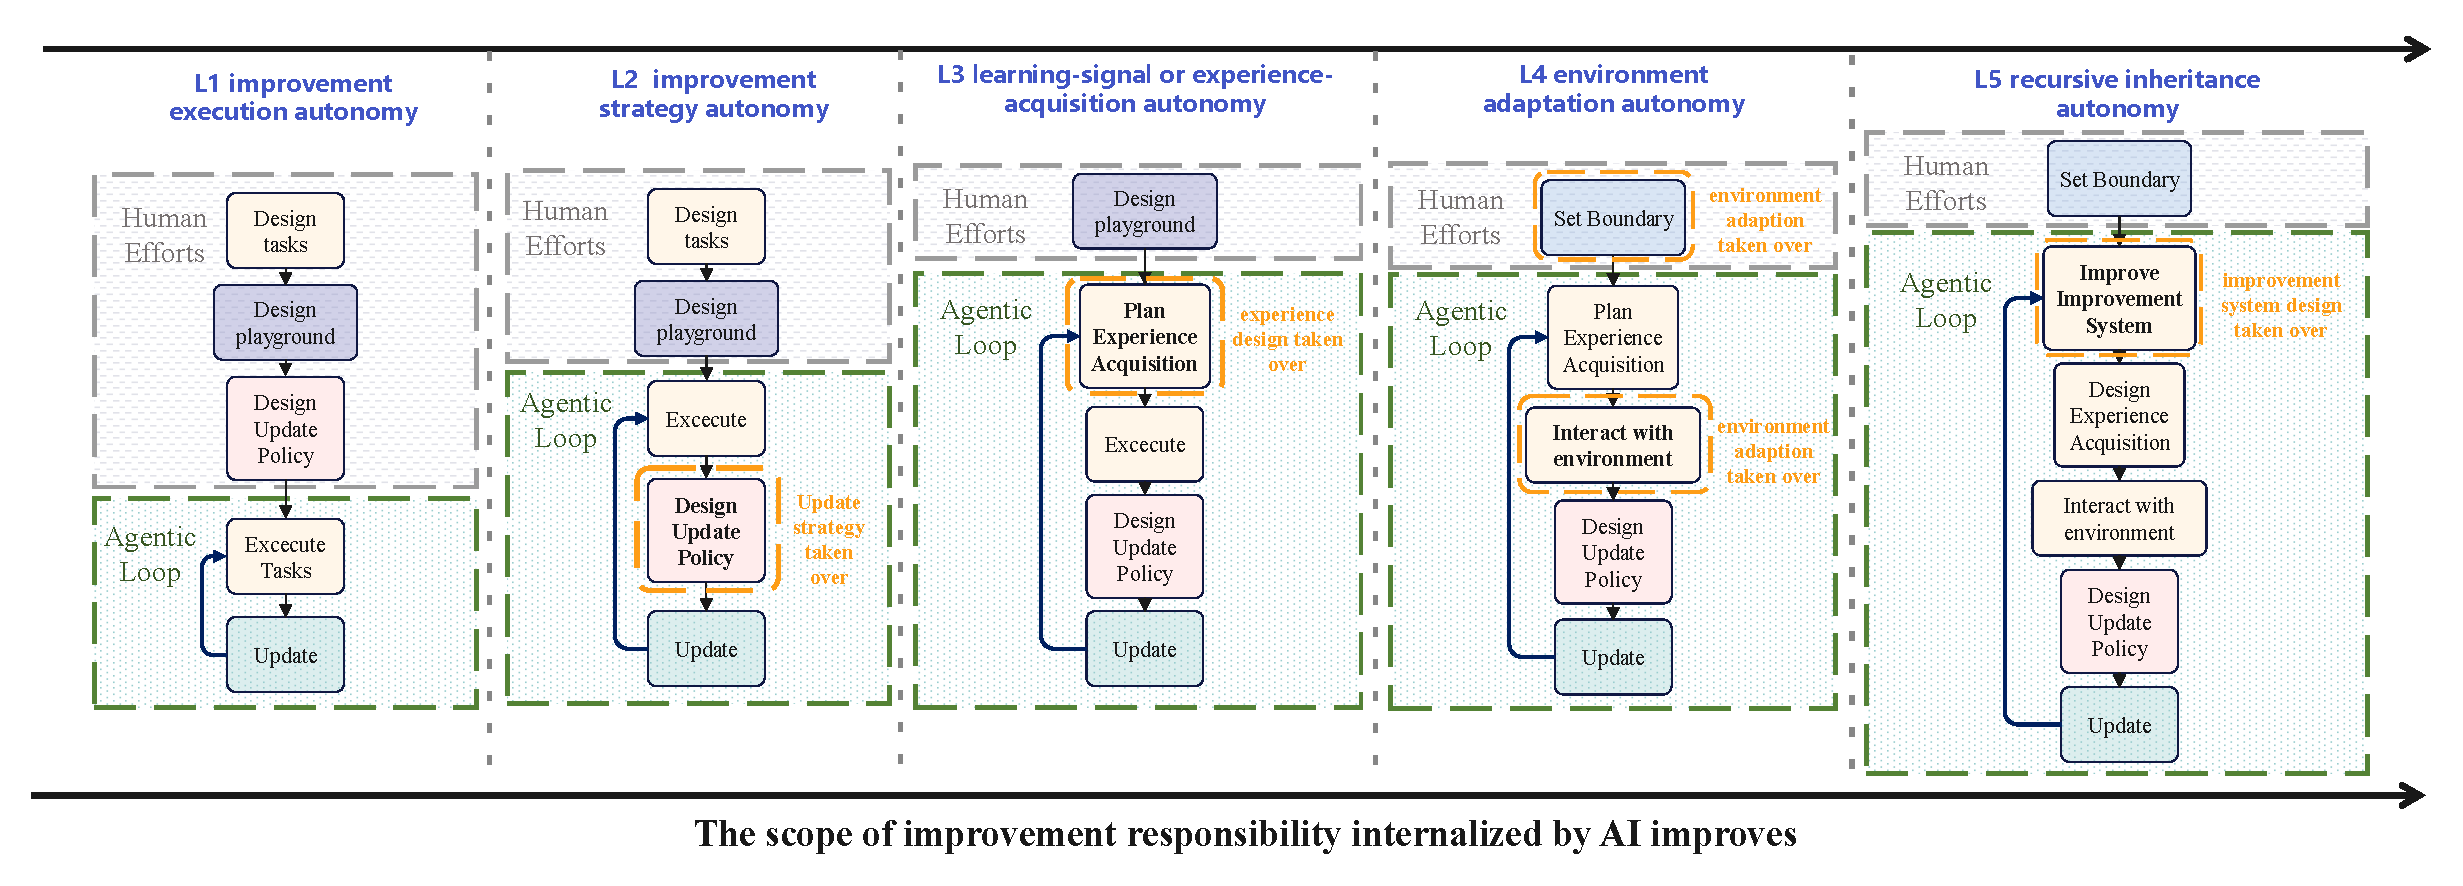
\includegraphics[width=1\linewidth]{figures/Fig3loop_ver9.10.pdf}
    \caption{Loop Patterns of Five Levels. Gray dashed frames indicate human-controlled components. Green dashed frames indicate components within the RSI loop. Orange outlines highlight the newly internalized component at each level. The expanding green frames show that AI progressively automates a larger share of the improvement process.} % Block colors indicate functional roles: yellow for experience acquisition, purple for playground design, red for update-policy design, green for update execution, and blue for boundary setting.
    \label{fig:five-loops}
\end{figure*}

\noindent$\bullet$ \textbf{(L1) Improvement Execution Autonomy.} Humans specify what should be improved, how it should be improved, and what constitutes success, while AI executes candidate updates. For example, FineWeb-Edu uses a model to apply human-defined educational-quality labels across a web corpus without choosing the labeling criterion~\cite{penedo2024fineweb}.

\noindent$\bullet$ \textbf{(L2) Improvement Strategy Autonomy.} The objective, task boundary, and evaluation criteria remain externally fixed, but AI diagnoses weaknesses and decides how to improve the system. For example, Self-Harness uses execution traces to propose and test edits to its agent harness under a fixed benchmark and promotion rule~\cite{zhang2026selfharness}.

\noindent$\bullet$ \textbf{(L3) Learning-Signal or Experience-Acquisition Autonomy.} The system also determines the experience needed for its next improvement round. For example, SIMA 2 uses assessments of current behavior to generate later practice tasks that target observed skill weaknesses~\cite{deepmind2025sima2}.

\noindent$\bullet$ \textbf{(L4) Environment Adaptation Autonomy.} The improvement loop uses deployment interaction to revise persistent system state under external acceptance and governance rules. For example, PANDO admits or demotes reusable rules during a long-running interaction according to observed outcomes, so later actions inherit earlier experience~\cite{li2026pando}.

\noindent$\bullet$ \textbf{(L5) Recursive Inheritance Autonomy.} The system persistently revises a mechanism that governs subsequent improvement, such as an \Improver, \Verifier, or successor-generation procedure. For example, A-Evolve-Training revises its research policy after development scores fail to predict external gains and uses the revised policy to direct the next training round~\cite{shi2026aevolvetraining}.


% \noindent\todo{2.4 Typical Application Scenarios}

\subsection{Application Domains}

While the autonomy levels describe the structure of an improvement loop, their practical meaning depends on the feedback available in a domain, as the same retained update may be straightforward to test in software engineering and difficult to validate in a physical or clinical setting. We consider science, embodied intelligence, software engineering, and healthcare because they expose four distinct feedback regimes, including experimental evidence with uncertain attribution, physical interaction with costly trials, executable tests with incomplete specifications, and high-stakes outcomes under expert oversight. These regimes allow us to compare how feedback cost and reliability affect the retention and reuse of improvements.

\noindent$\bullet$ \textbf{(S1) RSI for Science.}
Scientific discovery involves open-ended exploration, costly experiments, and feedback that may not clearly identify the source of failure. We examine how accumulated evidence can improve scientific hypothesis modules, experimental agents, and reflection or improvement mechanisms, with attention to whether these changes support subsequent research beyond the current scientific result.

\noindent$\bullet$ \textbf{(S2) RSI for Embodied Intelligence.}
Embodied agents generate experience through their own actions, while failures may arise from interacting perception, planning, and control components. Physical trials also impose limits on exploration and repeatability. We examine the evolution of environments and curricula, skills and agent harnesses, policies and action models, and world models and evaluators, focusing on how interaction feedback supports validated improvements that can be reused in later tasks.

\noindent$\bullet$ \textbf{(S3) RSI for Software Engineering.}
Software engineering makes both the developed artifact and the developing agent accessible to executable modification and testing. We examine how repository feedback supports persistent changes to coding-agent implementations and harnesses, development experience and collaboration, and the improvement process itself. A central distinction is whether an update improves current task performance, the ability to produce stronger successors, or both.

\noindent$\bullet$ \textbf{(S4) RSI for Healthcare.}
Healthcare combines restricted opportunities for trial and error with delayed, heterogeneous feedback and improvements whose validity may depend on the patient population or institution. We examine the evolution of clinical memory and knowledge, reasoning strategies, and tools and workflows, emphasizing how reviewed experience can inform subsequent cases under explicit validation and oversight.

Across these domains, we compare what is updated, how feedback supports its retention, and which decisions remain externally controlled. This analysis connects the autonomy framework to application-specific evidence and identifies the gaps between demonstrated improvement mechanisms and fuller recursive improvement.
% \dy{The significance of \RSI{} becomes clearer when the improvement loop is embedded in environments where tasks, feedback, and failure modes continue to evolve after deployment. We therefore examine five application domains in which persistent self-improvement may provide qualitatively different advantages.}

% \dy{S1: RSI for Science}

% \dy{S2: RSI for Embodied Intelligence}

% \dy{S3: RSI for Software Engineering}

% % \dy{S4: RSI for Cybersecurity}

% \dy{S4: RSI for Healthcare}

% \noindent\todo{2.5 Best Practices}

\subsection{Industrial Evidence}

The domain analysis identifies the feedback and validation conditions that shape an improvement loop, while industrial systems show how these conditions are handled within operating pipelines, where integration and deployment constraints are immediate. We examine industrial practice because frontier improvement loops are not always first documented through conventional academic publications. Industrial materials, including technical reports, open-source systems, engineering blogs, model documentation, and deployed product infrastructures, often reveal system-level practices, such as evaluation pipelines, data flywheels, agent harnesses, automated experimentation, and deployment feedback loops, which are only partially represented in the academic literature. We use these materials to complement the research literature and to understand how self-improvement is implemented under real engineering constraints.

Building on the autonomy-centered framework and application analysis, we examine what responsibilities industrial systems assume for their own improvement and how these responsibilities vary across applications and engineering settings. We further analyze how constraints such as computational cost, feedback quality, and human involvement shape the organization of improvement loops and limit the attainable scope of autonomy. This perspective allows us to characterize both the mechanisms that have been demonstrated in deployed or production-oriented systems and the more ambitious visions of recursive improvement that remain to be validated, thereby clarifying the current progress and limitations of industrial \RSI{} practice. Figure~\ref{fig:rsi-landscape} reports the surveyed literature by autonomy level and improvement target, while Table~\ref{tab:industry-landscape} provides the corresponding landscape of industrial systems.


% \noindent\todo{3 Differences with Existing Surveys and Tutorials (e.g., in ICLR or KDD)}

% Existing surveys systematically review self-improving and self-evolving systems from different perspectives. Gao et al.~\cite{gao2026selfevolving} organize the literature around evolution targets, timing, and mechanisms, alongside applications and evaluation. Ren et al.~\cite{ren2026selfimprovements} provide a unified formulation of foundation-model and agent-harness updates, organizing technical approaches by update targets and feedback sources. These works provide a foundation for understanding the composition and operation of self-improvement methods and highlight persistent state beyond model parameters as an important object of study.

% Recent surveys more directly concerned with \RSI\ further examine system autonomy and the evidence required to support improvement claims. Liu et al.~\cite{liu2026path} introduce a capability hierarchy ranging from manual improvement to general recursive self-improvement and organize the literature around system components and their co-improvement. Wang et al.~\cite{wang2026diving} classify evolution depth according to the objects affected by updates and connect each level to corresponding requirements for independent verification. Chen et al.~\cite{chen2026recursiveselfimprovement} analyze existing work along the dimensions of improvement targets and loop closure, with particular attention to evaluation mechanisms. These studies share our interest in persistent updates, recursive mechanisms, and reliability. The differences primarily concern the basis of classification and how it organizes the subsequent analysis.

% Related tutorials and workshops provide complementary perspectives. The KDD 2025 tutorial \emph{Evaluation \& Benchmarking of LLM Agents}~\cite{mohammadi2025evaluationtutorial} organizes its discussion around evaluation objectives and processes, covering agent assessment and challenges in enterprise deployment. The ICLR 2026 workshop \emph{AI with Recursive Self-Improvement}~\cite{zhuge2026rsiworkshop} brings together research on system updates and evidence of improvement, addressing the design, evaluation, and governance of self-improvement methods. Building on these discussions, our survey adopts the responsibilities that systems assume for their own improvement as its central organizing principle.

% Specifically, we take the improvement loop as the basic unit of analysis and construct autonomy levels according to the scope of improvement responsibility transferred from external designers to AI systems. We distinguish the execution of prescribed improvement procedures from autonomous strategy selection. We then examine how responsibility extends to determining future learning experience and adapting persistently during deployment, and ultimately to modifying and inheriting mechanisms that govern subsequent improvement. At each level, we trace where the loop closes and what changes are retained, while identifying the critical decisions that remain externally controlled. This perspective distinguishes systems that use similar techniques or update the same components according to the improvement responsibilities they actually assume. We also examine the scope of autonomy separately from the effectiveness of improvement, particularly distinguishing structural evidence that a revised improvement mechanism is retained and reused from evidence that it produces better successors under comparable resource budgets.

% We further apply this perspective throughout our analysis of applications and industrial practice. Across application settings such as scientific discovery, we examine how feedback conditions shape the realization of improvement responsibilities and constrain the transfer of persistent updates to subsequent tasks. The industry section draws on technical reports and materials describing operational systems to examine how self-improvement mechanisms are organized under engineering constraints, while distinguishing demonstrated mechanisms from visions of recursive improvement that remain to be validated. By connecting autonomy levels to concrete operating conditions, the survey provides an integrated analysis of the improvement responsibilities assumed by current systems, how these responsibilities are implemented, and the extent to which existing evidence supports claims of recursive improvement.

\subsection{Differences from Existing Surveys}

Existing surveys provide complementary taxonomies of self-evolving systems and the mechanisms from which improvement loops are built. These works establish much of the technical vocabulary on which our analysis relies. Our survey differs in four respects.

\noindent$\bullet$ \emph{Improvement loop as the unit of analysis.} Prior surveys organize work by stages of self-evolution, update objects, timing, or technical mechanisms~\cite{tao2024selfevolution,gao2026selfevolving,fang2025selfevolving,ren2026selfimprovements}. These views explain what changes and how the change is produced, but systems that update the same component may assign very different decisions to AI. We trace a complete loop: what triggers improvement, who proposes and validates a change, what persists, and which later decisions use the retained change.

\noindent$\bullet$ \emph{Responsibility as the autonomy criterion.} Related frameworks examine capability levels, co-evolution, dynamic agent state, and AI-for-AI systems~\cite{liu2026path,zong2026coevolution,xu2026dynamicgraph,ye2026ai4ai}. We operationalize autonomy through the improvement decisions transferred from external designers to the AI rather than through model capability or the number of automated components. Our five levels distinguish responsibility for execution, strategy selection, experience acquisition, environmental adaptation, and recursive inheritance.

\noindent$\bullet$ \emph{Separate evidence for recursion and performance.} Evaluation surveys study model-based judgment, agent assessment, rubric-guided learning, and oversight failures~\cite{li2025judge,yehudai2026evaluation,shan2026rubric,kim2024superalignment,slattery2024risk}. Higher task performance alone does not show that an improvement mechanism was revised, retained, and reused. We distinguish structural recursion, in which a revised improvement mechanism governs a later round, from effective recursion, in which that mechanism produces stronger successors under comparable budgets and independent evaluation.

\noindent$\bullet$ \emph{Mechanisms compared across operating conditions.} Work on correction, synthetic data, lifelong learning, memory, prompt optimization, and workflow design explains how individual components improve~\cite{pan2024correction,venktesh2025verification,niu2026testtime,long2024synthetic,zheng2026lifelong,huang2026memory,zhou2026externalization,ramnath2025prompt,lee2025compound,yue2026workflow,li2026environment}. We examine how these mechanisms function within complete loops across science, embodied intelligence, software engineering, healthcare, and industrial practice, where feedback cost, validation, and external control differ~\cite{ding2026verificationgap,zhou2026coding,zhu2026clinical}. Comparing the same loop questions across these settings reveals when a method depends on cheap executable feedback, repeated interaction, expert review, or production infrastructure.

These choices together position the survey between a catalog of improvement mechanisms and a general hierarchy of AI capabilities. Our aim is to determine which parts of an improvement loop current systems can assume, how retained changes affect later rounds, and what evidence supports claims of recursive progress.


\iffalse

\noindent\todo{1.1 Problems in foundation model training}

\zxh{--(haodong) We need to run the numbers on this from an economic standpoint.} 

\zxh{Right now, all these advances in model capabilities are built on massive compute, human labor, and data budgets. That approach is not what truly drives real model evolution. }

\subsection{Data annotation and evaluation}
Expert adjudication remains a constraint after annotation inference becomes inexpensive. Yext's Label Studio deployment~\cite{labelstudio2026yext} estimated \$16,000 in labor savings from \$150 of inference when replacing a second annotator, yet projected only a 15\% reduction in total project duration. Its assumptions included four part-time annotators over two months, with model development costs excluded. The difference between component savings and elapsed-time savings limits claims of end-to-end automation. RSI must reduce unresolved disagreements on subsequent batches through retained corrections and improved sample selection. The case provides no longitudinal error-rate comparison establishing that this review burden declines autonomously.

\subsection{Software engineering}
Review and integration can erase coding-time savings. Despite training pipelines such as Qwen3-Coder~\cite{qwen2025coder}, with 7.5 trillion tokens and approximately 70\% code, METR's field experiment~\cite{metr2025developers} found 19\% longer completion times across 246 repository tasks performed by 16 experienced developers using early-2025 tools. The Darwin G\"odel Machine~\cite{sakana2025dgm} raised benchmark performance from 20\% to 50\% through agent-code modification with a fixed foundation model, leaving half the evaluated tasks unresolved. Retained repair strategies therefore need stronger regression checks and evidence of reduced review time across successive production changes. Benchmark improvement alone leaves the cost of maintaining those changes unmeasured.

\subsection{Mathematics}
Expensive solution generation and restricted verifier coverage constrain mathematical improvement. NVIDIA's AIMO-2 pipeline~\cite{nvidia2025aimo} used 540,000 problems, 3.2 million long-reasoning solutions, and 1.7 million tool-integrated solutions. AlphaEvolve~\cite{deepmind2025alphaevolve} improved best-known results on roughly 20\% of more than 50 selected problems. Its industrial results included a 23\% faster kernel, a 1\% reduction in Gemini training time, and a deployed scheduling heuristic recovering 0.7\% of Google's compute resources. These gains depend on automatically evaluable objectives. Extending RSI to broader mathematics requires affordable formalization and evidence that retained discoveries reduce the search cost of later problems.

\subsection{Scientific research and R\&D}
Experimental validation remains the limiting feedback channel. Google's AI co-scientist~\cite{gottweis2025coscientist} evaluated 15 open research goals with seven experts and investigated selected proposals experimentally, without disclosing full computational and laboratory costs. The AI Scientist-v2~\cite{yamada2025aiscientistv2} produced one submission above an ICLR workshop's average acceptance threshold among three human-selected submissions. That denominator measures manuscript evaluation, leaving experimental reproducibility and discovery yield unmeasured. Scientific RSI needs retained negative results to improve subsequent experiment selection, but these demonstrations provide no matched-budget estimate of additional validated discoveries per laboratory hour. Slow assays and uncertain outcome attribution prevent inexpensive, frequent update validation.

\subsection{Medicine}
Selected-case accuracy leaves clinical deployment costs and residual diagnostic errors unresolved. Microsoft's MAI-DxO~\cite{microsoft2025diagnosis} achieved 80\% accuracy against a 20\% physician average on a 304-case sequential-diagnosis benchmark, with 20\% lower estimated diagnostic expenditure in a reported configuration. The remaining error rate was therefore 20\%, and the cost comparison excluded model development and prospective deployment. Learning from outcomes is further complicated by treatment effects and delayed follow-up. Clinical RSI must show that retained corrections lower errors on subsequent patients while reducing total supervision and investigation costs. These benchmark results provide no prospective patient-outcome estimate supporting that transition.

\subsection{Law}
Complete-work-product reliability remains low despite substantial reasoning expenditure. Harvey's initial Legal Agent Benchmark~\cite{harvey2026lab} reported approximately \$50.90 and 22 minutes per task for its leading configuration, with only 7.1\% meeting every rubric criterion. Thus, 92.9\% failed at least one criterion, although this does not measure the time needed to correct them. Persistent reuse of lawyer-approved corrections could reduce repeated research, but jurisdiction changes, confidential facts, and invalid citations complicate transfer across matters. Legal RSI must demonstrate a higher full-pass rate and lower combined drafting and review cost on new matters. The reported inference price excludes that unresolved professional workload.

\subsection{Finance and investment}
Numerical reliability is the immediate barrier to delegating financial models. Vals AI's Excel Modeling Benchmark~\cite{vals2026excel} reported leading configurations around 72--74\% at approximately \$6--12 per task. Its leading system passed 88\% of formula checks but only 63\% of numerical checks, leaving 37\% of numerical checks unsatisfied. Agentic Context Engineering~\cite{zhang2025ace} improved financial benchmark results by an average of 8.6 percentage points through evolving context, without establishing production review savings. RSI must preserve verified calculation procedures and detect dependent errors before workbook acceptance. Investment applications additionally require prospective returns after transaction costs, since these modeling scores provide no measure of trading advantage.

\subsection{Accounting and audit}
Improved classification can incur disproportionate execution cost. Digits' vendor benchmark~\cite{digits2026benchmark} raised the best general-purpose model from approximately 81\% to 87\% accuracy with skills and tools, while enhanced workflows were 5--22 times slower and consumed 8--19 times more resources. Its own ledger system reported 97.8\% accuracy with sub-second turnaround on 2,000 transactions. Even that rate corresponds to approximately 44 misclassifications per 2,000 transactions, calculated from the reported accuracy. This is a transaction count, not a financial-materiality estimate. RSI must reduce recurring exceptions and reconciliation work across reporting periods. Classification results leave accrual judgments, audit evidence, and complete closing accuracy untested.

\subsection{Consulting and enterprise knowledge work}
Research quality can require substantially greater inference expenditure. Anthropic's production Research system~\cite{anthropic2025research} improved its internal evaluation score by 90.2\% over a single-agent system, while multi-agent workflows used roughly 15 times the tokens of ordinary chat. These comparisons have different baselines and cannot establish cost-effectiveness. Agent-rewritten tool descriptions reduced subsequent completion time by 40\%, demonstrating a reusable improvement, but the report did not establish repeated autonomous improvement of the update process. For consulting, the missing evidence is lower combined analyst and model cost per accepted recommendation, including source verification and client revisions. Internal research scores do not measure subsequent implementation value.

\subsection{Professional writing}
Editorial quality and review effort remain poorly measured in production disclosures. Jasper's 2025 report~\cite{jasper2025review} recorded 2.5 million campaign assets, over 69,500 user-created Brand Voices, and more than 26,600 audience profiles. These are usage and configuration counts, with no corresponding factual-error rate, editing time per asset, or matched human-quality comparison. Consequently, they cannot quantify an autonomous writing advantage. Writing RSI must retain factual corrections and editorial decisions in ways that reduce substantive edits on later documents. The obstacle is obtaining reliable feedback from publication approvals, which can reflect deadlines and commercial priorities as well as accuracy.

\subsection{Creative media and design}
Production speed leaves originality and selection cost unresolved. Adobe's Firefly customer cases~\cite{adobe2025firefly} reported 270 banner variants produced by Monks in one day and a StudioRx rebranding completed in weeks against an estimated conventional duration of months. Neither comparison reports an acceptance denominator or total designer and generation expenditure. The resulting evidence supports faster asset production, with no quantified innovation advantage. Creative RSI needs retained acceptance and rejection feedback to reduce unsuccessful generation. Its remaining measurement problem is separating design quality from audience targeting and distribution when campaign response becomes the feedback signal.

\subsection{Translation and localization}
Compute efficiency and translation-review efficiency remain separate constraints. DeepL's engineering report~\cite{deepl2025fp8} described 544 H100 GPUs and a 1.5-billion-parameter training comparison using three trillion tokens. FP8 increased training throughput by approximately 50\% and roughly doubled inference throughput at comparable latency. In the CHORUS research prototype~\cite{wang2026chorus}, 30 licensed translators completed work 33.8\% faster than with single-agent assistance, using revision memory and specialized agents together. The memory component's independent contribution was unresolved. Translation RSI must demonstrate durable reductions in post-editing effort while controlling omissions and terminology conflicts across clients, with rare mistranslations included in quality assessment.

\subsection{Cybersecurity}
Discovery still exceeds successful repair. In the 2025 AI Cyber Challenge~\cite{darpa2025aixcc}, systems found 54 of 63 synthetic vulnerabilities and patched 43, leaving 20 unpatched, or approximately 32\% of the total. They also found 18 previously unknown real vulnerabilities and supplied 11 patches. Average execution cost was approximately \$152 per task and patch submission time averaged 45 minutes, alongside \$1.05 million in combined finalist-development model credits from three providers. The credits and execution costs represent separate budgets. Security RSI must retain validated failures and repair strategies while improving regression coverage. These aggregate competition results do not measure declining cost or improved repair rates across independent production campaigns.

\subsection{Robotics and embodied intelligence}
Demonstration demand and physical reliability constrain deployment. Figure's Helix~\cite{figure2025helix} increased demonstration data from 10 to 60 hours while reducing package-processing time from 6.84 to 4.31 seconds and raising barcode-orientation success from 88.2\% to 94.4\%. This represents sixfold data growth for a calculated 37\% cycle-time reduction, with 5.6\% orientation failures remaining. ReCAP~\cite{physicalintelligence2025recap} more than doubled throughput on some tasks using autonomous experience and expert corrections. RoboCasa365~\cite{nasiriany2026robocasa} raised real-world success from 61.8\% to 79.8\% through simulation pretraining, while the separate RoboDojo benchmark~\cite{robodojo2026benchmark} reported 12.8\% for its strongest policy against 100\% for expert teleoperators. These protocols are not directly comparable. Embodied RSI must reduce intervention and validation costs under hardware constraints, with no demonstrated orders-of-magnitude reduction in total iteration cost in these results.
\fi
